\section{What is \scalenetcdf File?} \label{sec:netcdf}

In this section, \scalenetcdf file, which \scalelib directly reads from and writes in, is explained.
\scalelib employs \netcdf (network Common Data Format) as data file format.
\Netcdf is a software developed by Unidata (\url{http://www.unidata.ucar.edu/}),
and it enables us to generate files with self-describing and machine-independent data format;
for example, the former has a merit to describe variables along with their axis variables in a file and
the latter has a merit to treat data without worry which endian is used.
Based on the above virtue, \scalelib has particular conversion ( \scalenetcdf convention ).
It is mostly following the CF conventions \\ (\url{http://cfconventions.org}).


\subsection{Global Attributes}
\scalenetcdf file contains information about data contained in the file,
such as those with regards to spatial decomposition as ``Global Attributes'' (Table \ref{table:netcdf_global_attrs}).

\begin{table}%[bth]
\begin{center}
  \caption{Global attributes in \scalenetcdf file}
  \label{table:netcdf_global_attrs}
  \begin{tabularx}{150mm}{p{50mm}XX} \hline
    Name        & Description                 & Remarks \\ \hline \hline
    title       & Brief description of data   & Value of \nmitem{FILE_History_TITLE} in \namelist{PARAM_FILE_HISTORY} \\
    source      & Name of the source software & Value of \nmitem{FILE_History_SOURCE} in \namelist{PARAM_FILE_HISTORY} for history files and \nmitem{H_SOURCE} in \namelist{PARAM_IO} for other files\\
    institution & Data author                 & Value of \nmitem{FILE_History_INSTITUTION} in \namelist{PARAM_FILE_HISTORY} for history files and \nmitem{H_INSTITUTE} for other files\\
    rankid      & Rank id of MPI process      & \verb|PRC_myrank| in the model \\
    Conventions & CF convention version       & ``CF-1.6'' for version 5.3 \\
    grid\_name  & Grid type                   & ``cartesC'' for \scalerm \\
    scale\_cartesC\_prc\_rank\_[xy]           & Mapping index of the 2D decomposition      & Equal to \verb|PRC_2Drank(PRC_myrank, i)| variable in the model (i=1 for x and 2 for y)\\
    scale\_cartesC\_prc\_num\_[xy]            & Number of the 2D decomposition             & ~\nmitem{PRC_NUM_X}, \nmitem{PRC_NUM_Y} in the model \\
    scale\_cartesC\_prc\_periodic\_[zxy]      & Whether the boundary condition is periodic & \verb|.false.| and \verb|.true.|\ They correspond to \nmitem{PRC_PERIODIC_X}, \nmitem{PRC_PERIODIC_Y} in the model\\
    scale\_atmos\_grid\_cartesC\ \_index\_[ij]maxg  & Number of the grids in the global domain               & ~\nmitem{IMAX} $\times$ \nmitem{PRC_NUM_X}, \nmitem{JMAX} $\times$ \nmitem{PRC_NUM_Y} in the model \\
    scale\_atmos\_grid\_cartesC\ \_index\_kmax      & Number of the vertical layer for the atmospheric model & ~\nmitem{KMAX} in the model \\
    scale\_ocean\_grid\_cartesC\ \_index\_kmax      & Number of the vertical layer for the ocean model       & ~\nmitem{OKMAX} in the model \\
    scale\_land\_grid\_cartesC\ \_index\_kmax       & Number of the vertical layer for the land model        & ~\nmitem{LKMAX} in the model \\
    scale\_urban\_grid\_cartesC\ \_index\_kmax      & Number of the vertical layer for the urban model       & ~\nmitem{UKMAX} in the model \\
    scale\_atmos\_grid\_cartesC\ \_index\_[kij]halo & Number of halo grids                                   & ~\nmitem{KHALO}, \nmitem{IHALO}, \nmitem{JHALO} in the model \\
    Calendar    & Calendar type                            & ~\nmitem{PARAM_CALENDAR} in the model \\
    time\_units & Unit of time & \\
    time\_start & Start time   & \\ \hline
    \multicolumn{3}{l}{Refer Section \ref{sec:output} for \nmitem{History_TITLE, History_SOURCE, History_INSTITUTION},} \\
    \multicolumn{3}{l}{Section \ref{sec:domain}       for \nmitem{PRC_NUM_X, PRC_NUM_Y, PRC_PERIODIC_X, PRC_PERIODIC_Y},} \\
    \multicolumn{3}{l}{\nmitem{KMAX, IMAX, JMAX}, and \ref{subsec:calendar} for \nmitem{PARAM_CALENDAR}.} \\ \hline
  \end{tabularx}
\end{center}
\end{table}



\subsection{Data in the Halo Region}

Whether the file 
contains the data in the halo region
depends on the type of file and its configuration.
Note that the halo region that we define here means the halo in the whole calculation region,
not the halo in each of local regions.

For the initial (or restart) and boundary data files, 
the halo data is contained if the lateral boundary conditions are not periodic 
(\nmitem{PRC_PERIODIC_X}, \nmitem{PRC_PERIODIC_Y} = .false. in \namelist{PARAM_PRC_CARTESC}) 
or the single file I/O (Section \ref{subsec:single_io}) is used (\nmitem{FILE_AGGREGATE}=.true. in \namelist{PARAM_FILE}),
otherwise it is not.

On the other hand,
for the history data file, 
the halo data is contained 
only when the lateral boundary conditions are not periodic
(\nmitem{PRC_PERIODIC_X}, \nmitem{PRC_PERIODIC_Y} = .false. in \namelist{PARAM_PRC_CARTESC})
and \nmitem{FILE_HISTORY_CARTESC_BOUNDARY}=.true. in \namelist{PARAM_FILE_HISTORY_CARTESC},
otherwise it is not. Refer Section \ref{sec:output} for detail.


\subsection{Axis Variables}
\scalenetcdf file contains axis data.
All the axis variables have 
``long\_name'' and ``units'' attributes,
which describe description and unit of the variable, respectively.
In addition, x, y, xh, and yh variables 
have attributes for the total number of grids in the whole domain (``size\_global''),
the start index in the total grid of data in the file (``start\_global''),
the number of the halo grids at the begin and end in the whole data (``halo\_global''),
and the number of the halo grids of data in the file (``halo\_local'').

Table \ref{table:netcdf_axes} shows list of the axis data.
The coordinate variables have their own dimension; their variable names are the same as their dimension names.
%The other axis variables use some dimensions of coordinate variables.
The variables with lower-case name are mainly used in the file, 
while those with the upper-case name describe axes in simulation.
Figure \ref{fig:netcdfhorizontalcoordinate} and \ref{fig:netcdfverticalcoordinate} show 
the horizontal and vertical locations of coordinate variables,
respectively.
Refer to them with Table \ref{table:netcdf_axes} at the same time.

The area and volume data of the grids are also in the file as ``cell\_area**'' and ``cell\_volume**'', respectively.
The ``cell\_measures'' attribute of each variables specifies the corresponding area or volume data.

The map projection data is contained as a non-dimensional variable whose name is specified by ``grid\_mapping'' attribute of the variables.

The information of relationship the staggered grids, an attribute and a non-dimensional variable are contained as follows SGRID conventions (\url{https://github.com/sgrid/sgrid}).
The non-dimensional variable's name is specified by the ``grid'' attribute of each variable.

In the file, there are also the surface elevation data and land mask data as ``topo'' and ``lsmask'', respectively.



\begin{longtable}{l|l}
  \caption{Axis data in \scalenetcdf .}
  \label{table:netcdf_axes} \\ \hline
  \endfirsthead
  \multicolumn{2}{l}{\small\it Cont.} \\ \hline
%  & name & description \\ \hline \hline
  \endhead
  \hline
  \endfoot
  \multicolumn{2}{l}{Coordinate variables}\\ \hline
name & description \\ \hline \hline
\multicolumn{2}{c}{Common : Horizontal axis \& time}\\ \hline
x        & full level position in x-direction of the data in the file \\
x\_bnds  & full level cell boundary in x-direction of the data in the file \\
xh       & half level position in x-direction of the data in the file \\
xh\_bnds & half level cell boundary in x-direction of the data in the file \\
y        & full level position in y-direction of the data in the file \\
y\_bnds  & full level cell boundary in y-direction of the data in the file \\
yh       & half level position in y-direction of the data in the file \\
yh\_bnds & half level cell boundary in y-direction of the data in the file \\
time       & time information \\ \hline
time\_bnds & time boundary information \\ \hline
CX  & full level grid position in x-direction for the local region (inc. halo grids) \\
FX  & half level grid position in x-direction for the local region (inc. halo grids) \\
CDX & full level grid spacing  in x-direction (inc. halo grids) \\
FDX & half level grid spacing  in x-direction (inc. halo grids) \\
CY  & full level grid position in y-direction for the local region (inc. halo grids) \\
FY  & half level grid position in y-direction for the local region (inc. halo grids) \\
CDY & full level grid spacing  in y-direction (inc. halo grids) \\
FDY & half level grid spacing  in y-direction (inc. halo grids) \\
CXG & full level grid position in x-direction for the whole region (inc. halo grids) \\
FXG & half level grid position in x-direction for the whole region (inc. halo grids) \\
CYG & full level grid position in y-direction for the whole region (inc. halo grids) \\
FYG & half level grid position in y-direction for the whole region (inc. halo grids) \\ \hline
\multicolumn{2}{c}{Vertical axis : Atmosphere}\\ \hline
z         & full level position in z-direction in the file \\
z\_bnds   & full level cell boundary in z-direction in the file \\
zh        & half level position in z-direction in the file \\
zh\_bnds  & half level cell boundary in z-direction in the file \\
CZ  & full level grid position in z-direction (inc. halo grids) \\
FZ  & half level grid position in z-direction (inc. halo grids) \\
CDZ & full level grid spacing  in z-direction (inc. halo grids) \\
FDZ & half level grid spacing  in z-direction (inc. halo grids) \\ \hline
\multicolumn{2}{c}{Vertical axis : Land}\\ \hline
oz        & full level position in z-direction of the ocean data in the file \\
oz\_bnds  & full level cell boundary in z-direction of the ocean data in the file \\
ozh       & half level position in z-direction of the ocean data in the file \\
ozh\_bnds & half level cell boundary in z-direction of the ocean data in the file \\
OCZ  & full level grid position in z-direction of the ocean model \\
OFZ  & half level grid position in z-direction of the ocean model \\
OCDZ & full level grid spacing in z-direction of the ocean model \\  \hline
\multicolumn{2}{c}{Vertical axis : Land}\\ \hline
lz        & full level position in z-direction of the land data in the file \\
lz\_bnds  & full level cell boundary in z-direction of the land data in the file \\
lzh       & half level position in z-direction of the land data in the file \\
lzh\_bnds & half level cell boundary in z-direction of the land data in the file \\
LCZ  & full level grid position in z-direction of the land model \\
LFZ  & half level grid position in z-direction of the land model \\
LCDZ & full level grid spacing in z-direction of the land model \\  \hline
\multicolumn{2}{c}{Vertical axis : Urban canopy}\\ \hline
uz        & full level position in z-direction in the file \\
uz\_bnds  & full level cell boundary in z-direction in the file \\
uzh       & half level position in z-direction in the file \\
uzh\_bnds & half level cell boundary in z-direction in the file \\
UCZ  & full level grid position in z-direction \\
UFZ  & half level grid position in z-direction \\
UCDZ & full level grid spacing in z-direction \\ \hline
 \hline
  \multicolumn{2}{l}{Other axis variables (1D)}\\ \hline
name  & description \\ \hline \hline
CBFZ  & buffer factor at CZ \\
FBFZ  & buffer factor at FZ \\
CBFX  & buffer factor at CX for the local region \\
FBFX  & buffer factor at FX for the local region \\
CBFY  & buffer factor at CY for the local region \\
FBFY  & buffer factor at FY for the local region \\
CBFXG & buffer factor at CXG for the whole region \\
FBFXG & buffer factor at FXG for the whole region \\
CBFYG & buffer factor at CYG for the whole region \\
FBFYG & buffer factor at FYG for the whole region \\
\hline
\multicolumn{2}{l}{Other axis variables (2D)}\\ \hline
name & description \\ \hline \hline
lon     & longitude at (y, x) \\
lon\_uy & longitude at (y, xh) \\
lon\_xv & longitude at (yh, x) \\
lon\_uv & longitude at (yh, xh) \\
lat     & latitude  at (y, x) \\
lat\_uy & latitude  at (y, xh) \\
lat\_xv & latitude  at (yh, x) \\
lat\_uv & latitude  at (yh, xh) \\
\hline
\multicolumn{2}{l}{Other axis variables (3D)}\\ \hline
name & description \\ \hline \hline
height      & heigth at (z, y, x)    in history file or at (y, x, z)    in restart/initial file\\
height\_xyw & height at (zh, y, x)   in history file or at (y, x, zh)   in restart/initial file\\
height\_xvz & height at (z, yh, x)   in history file or at (yh, x, z)   in restart/initial file\\
height\_uyz & height at (z, yh, xh)  in history file or at (hy, x, z)   in restart/initial file\\
height\_xvw & height at (zh, yh, x)  in history file or at (yh, x, zh)  in restart/initial file\\
height\_uyw & height at (zh, y, xh)  in history file or at (y, xh, zh)  in restart/initial file\\
height\_uvz & height at (z, yh, xh)  in history file or at (yh, xh, z)  in restart/initial file\\
height\_uvw & height at (zh, yh, xh) in history file or at (yh, xh, zh) in restart/initial file\\
\end{longtable}



\begin{figure}[tbh]
\begin{center}
  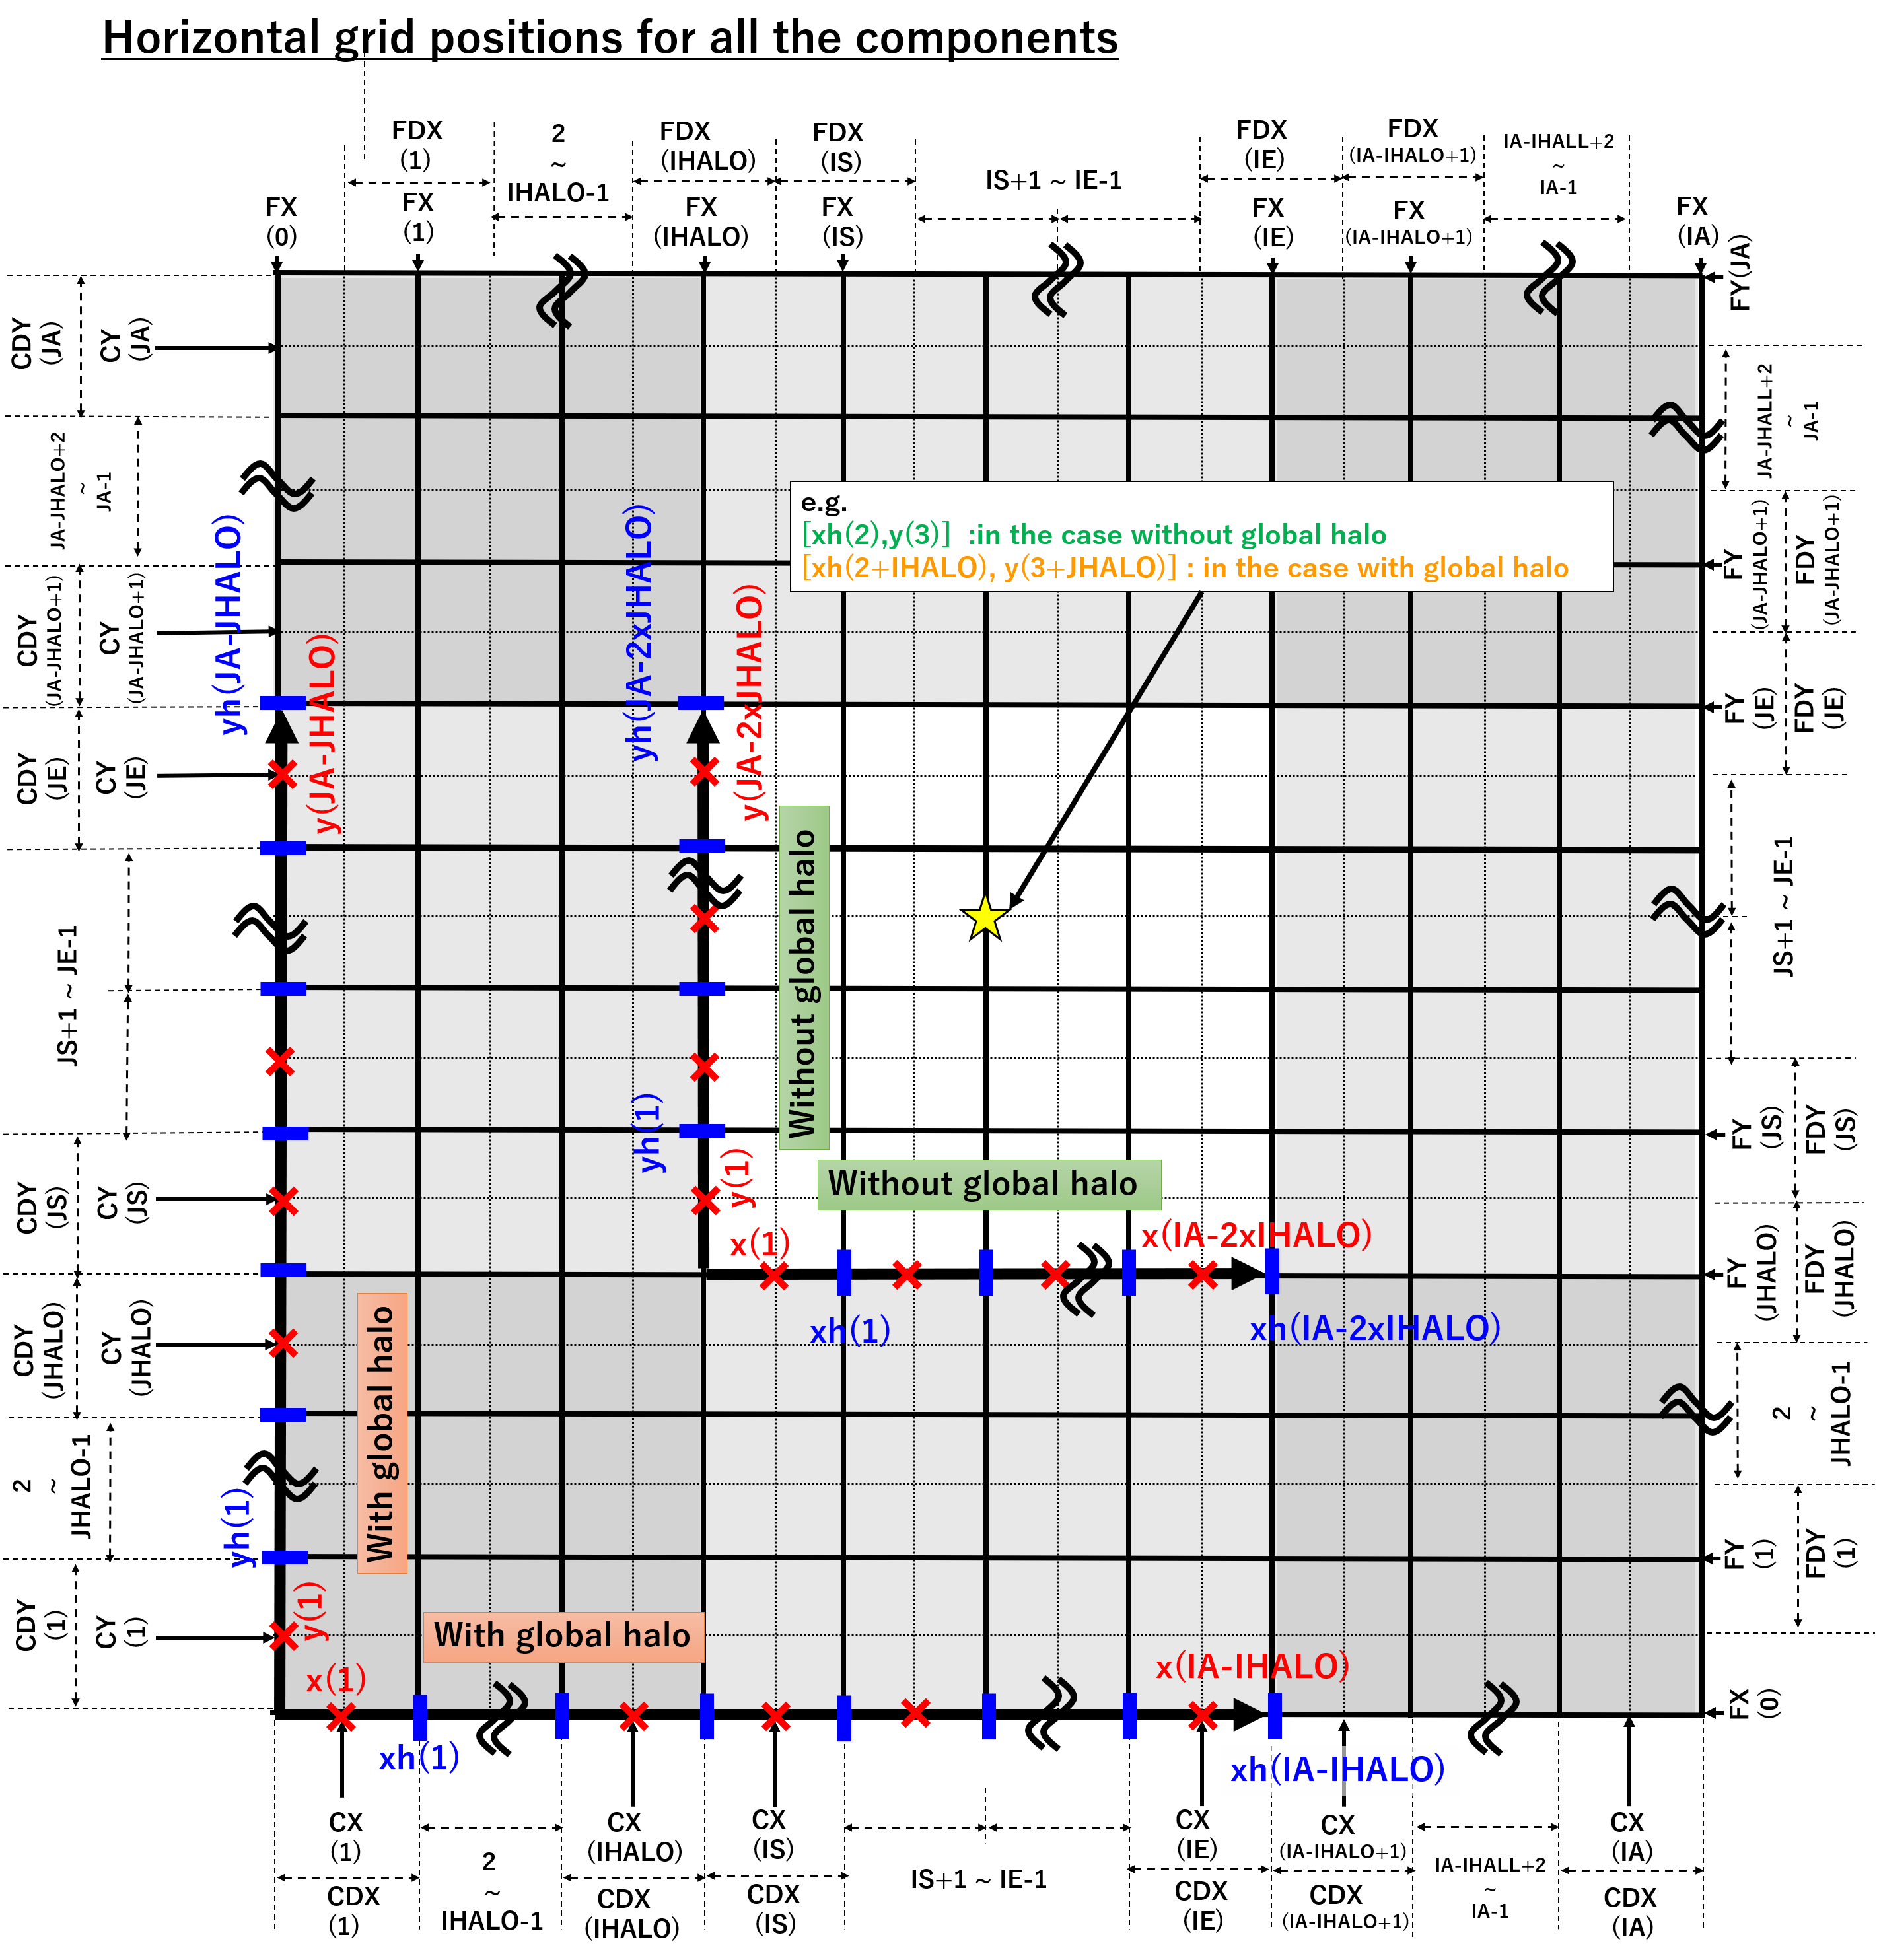
\includegraphics[width=1.0\hsize]{./figure/horizontal-coordinate-final2.png}\\
  \caption{Horizontal coordinate in {\scalenetcdf} file}
  \label{fig:netcdfhorizontalcoordinate}
\end{center}
\end{figure}
\begin{figure}[tbh]
\begin{center}
  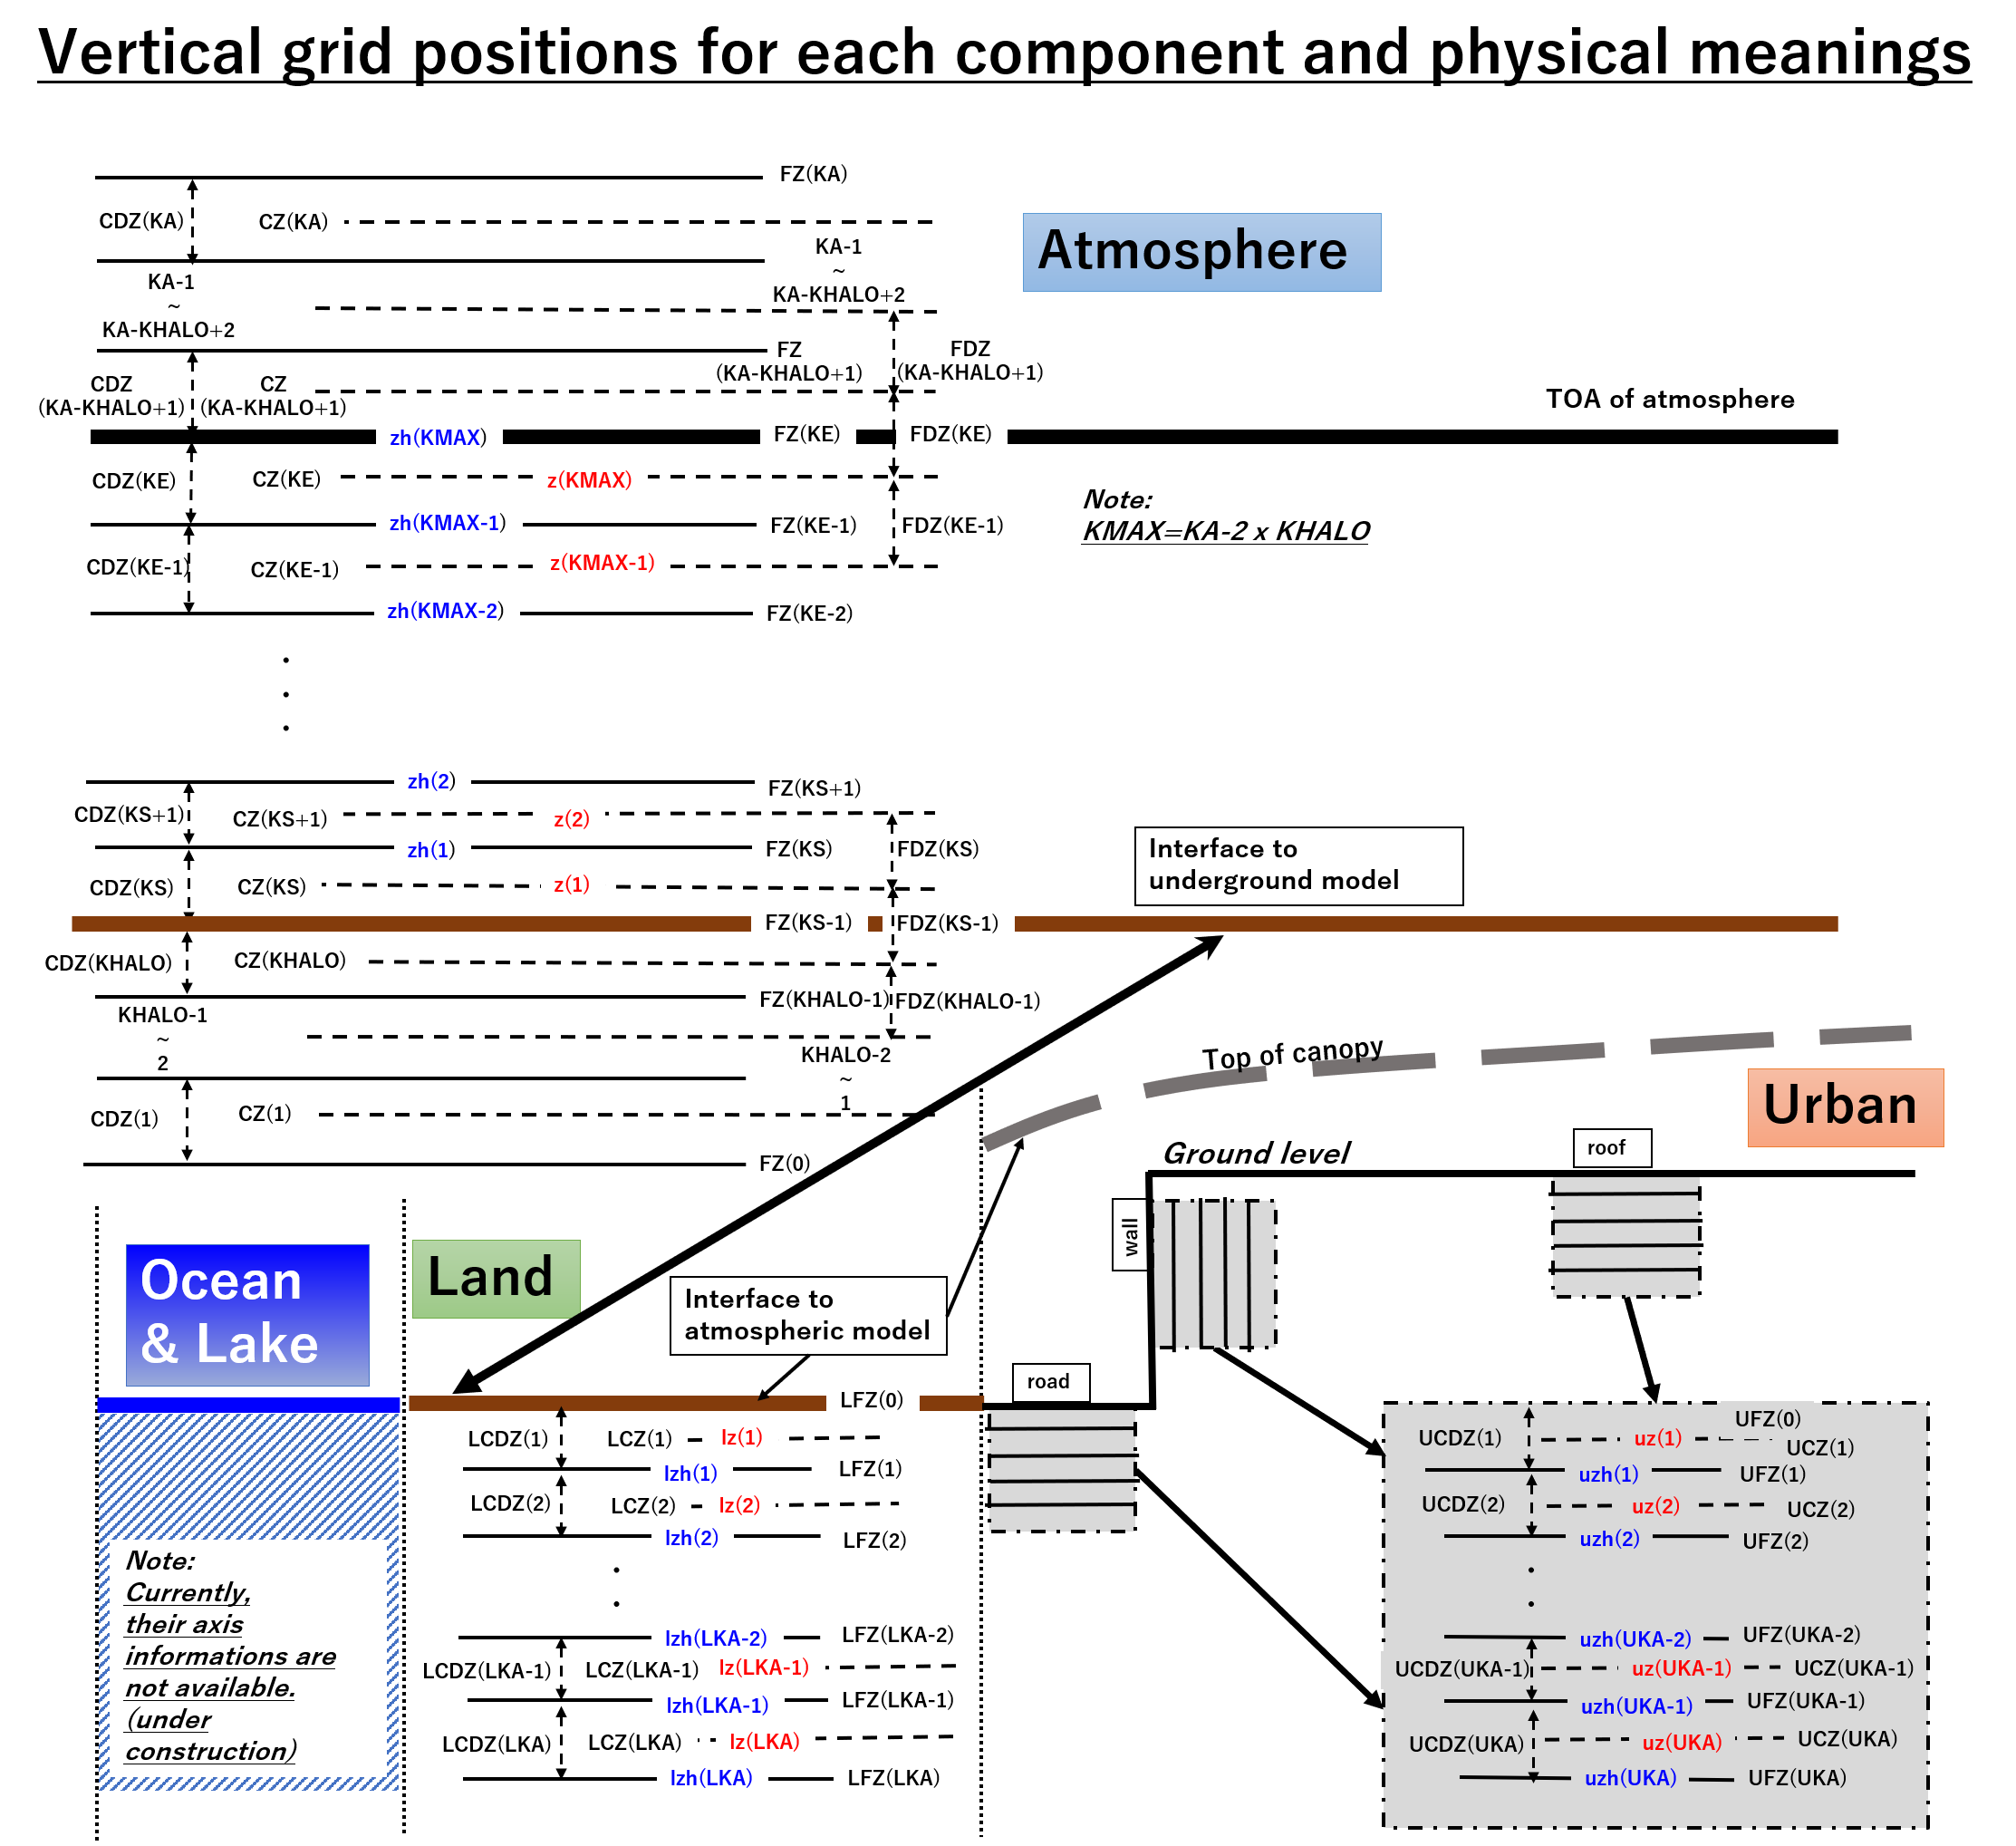
\includegraphics[width=1.0\hsize]{./figure/vertical_coordinate_final2.png}\\
  \caption{Horizontal coordinate in {\scalenetcdf} file}
  \label{fig:netcdfverticalcoordinate}
\end{center}
\end{figure}



\subsection{Data Variables}
Data variables have attributes of the undefined value ``\_FillValue'' and 
the missing value ``missing\_value'' as well as ``long\_name'' and ``untis''.
Data structure in the initial (restart) data and boundary data files 
is identical to the array in the model, that is the z-x-y order.
On the other hand, it in the history data file is the x-y-z order.
This is true for 3D axis variables.
See also Table \ref{table:netcdf_axes}.



\subsection{Single File I/O} \label{subsec:single_io}
As default, all the data files are output by each process, namely separate file I/O.
If \scalerm is compiled with pnetCDF (environmental variable SCALE\_ENABLE\_PNETCDF=T),
the data from all processes can be combined into a single file (See Section \ref{subsec:environment}).
To do this, set \nmitem{FILE_AGGREGATE} in \namelist{PARAM_FILE}) \verb|.true.|. The all the data files become single file.
In stead, you can switch on/off of the single I/O for individual file types, i.e., history, init/restart, topography, and land use files.
Set \nmitem{FILE_HISTORY_AGGREGATE}=.true. in \namelist{PARAM_FILE_HISTORY} for the history file.
For init/restart files, set \nmitem{RESTART_(IN|OUT)_AGGREGATE}=.true. in \namelist{PARAM_RESTART},\\
or \nmitem{(MODELNAME)_RESTART_(IN|OUT)_AGGREGATE}=.true. in \namelist{PARAM_(MODELNAME)_VARS}.
Here, \verb|(MODELNAME)| is ``ATMOS'', ``OCEAN'', ``LAND'', or ``URBAN''.
For topography and land use files, set \nmitem{TOPO_(IN|OUT)_AGGREGATE}=.true. in \namelist{PARAM_TOPO} and \nmitem{LANDUSE_(IN|OUT)_AGGREGATE}=.true. in \namelist{PARAM_LANDUSE}, respectively.


\subsection{Restrictions with \Netcdf 3}
If \scale is compiled with \netcdf version 3, the following restrictions exist.
\begin{itemize}
\item Variables with different time intervals cannot stored in the same file.
\item Compression of data cannot be used.
\item File of {\netcdf}4 format cannot be read.
\end{itemize}
If you want to output variables with different time intervals, set \nmitem{BASENAME} in \namelist{HISTORY_ITEM} to output them to different files.

Note that the restrictions of the multiple time interval and compression are placed when the single file I/O is used,
because pnetCDF is based on \netcdf 3 file format.

\begin{table}
  \caption{Functionality of each \netcdf versions.}
  \begin{tabular}{llllll} \hline
    & \shortstack{multiple\\time interval} & Compression & \shortstack{Read\\\netcdf 3 file} & \shortstack{Read\\\netcdf 4 file} & \shortstack{Read\\single file}\\ \hline
    \netcdf 3 & NG & NG & OK & NG & NG$^{*}$ \\
    \netcdf 4 & OK & OK & OK & OK & NG$^{*}$ \\
    pnetCDF   & NG & NG & NG$^{*}$ & NG & OK \\\hline
  \end{tabular}
  \\
  (*) it is OK if the number of total processes is 1.
\end{table}
